\documentclass[12pt,twoside]{report}
\usepackage[utf8x]{inputenc}

%%%%%%%%%%%%%%%%%%%%%%%%%%%%%%%%%%%%%%%%%%%%%%%%%%%%%%%%%%%%%%%%%%%%%%%%%%%%%

% Definitions for the title page
% Edit these to provide the correct information
% e.g. \newcommand{\reportauthor}{Timothy Kimber}

\newcommand{\reporttitle}{Evaluation of various entangling gates for trapped ion quantum computers}
\newcommand{\projectcode}{QOLS-Thompson-1}
\newcommand{\supervisor}{Prof. Richard Thompson}
\newcommand{\degreetype}{MSci Physics}
%\newcommand{\partner}{Zhang Rongjie}
\newcommand{\CID}{01496799}
\newcommand{\assessor}{Dr. Steve Kolthammer}

%%%%%%%%%%%%%%%%%%%%%%%%%%%%%%%%%%%%%%%%%%%%%%%%%%%%%%%%%%%%%%%%%%%%%%%%%%%%%

% load some definitions and default packages
%%%%%%%%%%%%%%%%%%%%%%%%%%%%%%%%%%%%%%%%%
% University Assignment Title Page 
% LaTeX Template
% Version 1.0 (27/12/12)
%
% This template has been downloaded from:
% http://www.LaTeXTemplates.com
%
% Original author:
% WikiBooks (http://en.wikibooks.org/wiki/LaTeX/Title_Creation)
%
% License:
% CC BY-NC-SA 3.0 (http://creativecommons.org/licenses/by-nc-sa/3.0/)
% 
%
%%%%%%%%%%%%%%%%%%%%%%%%%%%%%%%%%%%%%%%%%
%----------------------------------------------------------------------------------------
%	PACKAGES AND OTHER DOCUMENT CONFIGURATIONS
%----------------------------------------------------------------------------------------
\usepackage[a4paper,hmargin=2.5cm,vmargin=2cm,includeheadfoot]{geometry}
\usepackage{textpos}
\usepackage{cite} % for bibliography
\usepackage{tabularx,longtable,multirow,subcaption,caption,wrapfig}%hangcaption
\usepackage{fncylab} %formatting of labels
\usepackage{fancyhdr} % page layout
\usepackage{url} % URLs
\usepackage[english]{babel}
\usepackage{amsmath}
\usepackage{amsfonts}
\usepackage{graphicx}
\usepackage{dsfont}
\usepackage{epstopdf} % automatically replace .eps with .pdf in graphics
\usepackage{backref} % needed for citations
\usepackage{array}
\usepackage{latexsym}
\usepackage[pdftex,pagebackref,hypertexnames=false,colorlinks]{hyperref} % provide links in pdf

\hypersetup{pdftitle={},
  pdfsubject={}, 
  pdfauthor={},
  pdfkeywords={}, 
  pdfstartview=FitH,
  pdfpagemode={UseOutlines},% None, FullScreen, UseOutlines
  bookmarksnumbered=true, bookmarksopen=true, colorlinks,
    citecolor=black,%
    filecolor=black,%
    linkcolor=black,%
    urlcolor=black}

\usepackage[all]{hypcap}


%\usepackage{color}
%\usepackage[tight,ugly]{units}
%\usepackage{float}
%\usepackage{tcolorbox}
%\usepackage[colorinlistoftodos]{todonotes}
% \usepackage{ntheorem}
% \theoremstyle{break}
% \newtheorem{lemma}{Lemma}
% \newtheorem{theorem}{Theorem}
% \newtheorem{remark}{Remark}
% \newtheorem{definition}{Definition}
% \newtheorem{proof}{Proof}


%%% Default fonts
\renewcommand*{\rmdefault}{bch}
\renewcommand*{\ttdefault}{cmtt}



%%% Default settings (page layout)
\setlength{\parindent}{0em}  % indentation of paragraph

\setlength{\headheight}{14.5pt}
\pagestyle{fancy}
\renewcommand{\chaptermark}[1]{\markboth{\chaptername\ \thechapter.\ #1}{}} 

\fancyfoot[ER,OL]{\sffamily\textbf{\thepage}}%Page no. in the left on odd pages and on right on even pages
\fancyfoot[OC,EC]{\sffamily }
\renewcommand{\headrulewidth}{0.1pt}
\renewcommand{\footrulewidth}{0.1pt}
\captionsetup{margin=10pt,font=small,labelfont=bf}


%--- chapter heading

\def\@makechapterhead#1{%
  \vspace*{10\p@}%
  {\parindent \z@ \raggedright \sffamily
    \interlinepenalty\@M
    \Huge\bfseries \thechapter \space\space #1\par\nobreak
    \vskip 30\p@
  }}

%---chapter heading for \chapter*  
\def\@makeschapterhead#1{%
  \vspace*{10\p@}%
  {\parindent \z@ \raggedright
    \sffamily
    \interlinepenalty\@M
    \Huge \bfseries  #1\par\nobreak
    \vskip 30\p@
  }}

\allowdisplaybreaks

\newcommand{\der}[3][]{\frac{\text{d}^{#1}#2}{\text{d}#3^{#1}}}
\newcommand{\partder}[3][]{\frac{\partial^{#1}#2}{\partial#3^{#1}}}
\newcommand{\expon}[2]{#1\cdot 10^{#2}}
\newcommand{\figref}[1]{Figure \ref{#1}}
\newcommand{\eref}[1]{Equation \eqref{#1}}
\newcommand{\tabref}[1]{Table \ref{#1}}
\newcommand{\result}[3]{$#1 \pm #2\,\text{#3}$}
\newcommand{\resexp}[4]{$\expon{(#1 \pm #2)}{#4}\,\text{#3}$}
\newcommand{\absresult}[3]{$\mathbf{#1 \pm #2\,\text{#3}}$}
\newcommand{\absresexp}[4]{$\mathbf{\expon{(#1 \pm #2)}{#4}\,\text{#3}}$}

\usepackage[export]{adjustbox}
\usepackage{pdfpages}
\usepackage{pgf}
\usepackage{relsize}
\usepackage{hyperref}

\graphicspath{{Images/}}

% load some macros
%\input{notation}

\date{May 2022}

\begin{document}

% load title page
% Last modification: 2015-08-17 (Marc Deisenroth)
\begin{titlepage}

\newcommand{\HRule}{\rule{\linewidth}{0.5mm}} % Defines a new command for the horizontal lines, change thickness here


%----------------------------------------------------------------------------------------
%	LOGO SECTION
%----------------------------------------------------------------------------------------


\includegraphics[width = 6cm]{./imperial}\\[0.5cm] 

\center % Center remainder of the page

%----------------------------------------------------------------------------------------
%	HEADING SECTIONS
%----------------------------------------------------------------------------------------

\textsc{\Large Imperial College London}\\[0.5cm] 
\textsc{\large Department of Physics}\\[0.5cm] 

%----------------------------------------------------------------------------------------
%	TITLE SECTION
%----------------------------------------------------------------------------------------

\HRule \\[0.4cm]
{ \huge \bfseries \reporttitle}\\ % Title of your document
\HRule \\[1.5cm]
 
%----------------------------------------------------------------------------------------
%	AUTHOR SECTION
%----------------------------------------------------------------------------------------

\begin{minipage}{0.4\textwidth}
\begin{flushleft} \large
\emph{Author CID:}\\
\CID\\
\vspace*{1em}
\emph{Project code:}\\
\projectcode
\end{flushleft}
\end{minipage}
~
\begin{minipage}{0.4\textwidth}
\begin{flushright} \large
\emph{Supervisor:} \\
\supervisor\\ % Supervisor's Name
\vspace*{1em}
\emph{Assessor:}\\
\assessor
\end{flushright}
\end{minipage}\\[4cm]

\vspace*{2em}
\begin{center}
	\emph{Word Count:}\\
	8019
\end{center}

%----------------------------------------------------------------------------------------
%	FOOTER & DATE SECTION
%----------------------------------------------------------------------------------------
\vfill % Fill the rest of the page with whitespace
Submitted as part of 
\degreetype~degree of Imperial College London\\[0.5cm]

\makeatletter
\@date 
\makeatother


\end{titlepage}




% page numbering etc.
\pagenumbering{roman}
\clearpage{\pagestyle{empty}\cleardoublepage}
\setcounter{page}{1}
\pagestyle{fancy}

\fancyhead[RE,LO]{\sffamily {\large\textbf{Improving the reliability of trapped ion quantum computers}}}

{%\small
\vspace*{-2.em}
The weird world of quantum physics may be the next breakthrough in computation. But what can quantum computers do that classical ones cannot? Exploiting their unique properties we can create more efficient algorithms for many computational challenges. The most well known example is integer factorisation for which the runtime on classical computers scales as an exponential function of the size of the number being factorised. This exponential increase however can be overcome by using Shor's algorithm, which can only be implemented on quantum computers.

A classical computer's internal state can be represented as a series of bits, each of which can be $0$ or $1$. The difference in quantum computers is that it stores data in qubits, the quantum analogue of the bit. While only measured as either $0$ or $1$ the outcome of measuring a qubit is probabilistic and in between measurements we can manipulate these probabilities. This state where we are uncertain about the state we'll see when we measure the qubit is referred to as superposition. The most important thing however is that this probability can also be conditional on the state of other qubits in our computer, which is referred to as entanglement. As an example, with two qubits one can create something called a Bell state, where there is an equal probability of measuring each qubit as $0$ or $1$, but either of them is measured $0$ then the other one will be guaranteed $0$ as well. Conversely, if either of them is measured as $1$, then the other will be $1$.

\begin{wrapfigure}{r}{0.4\linewidth}
	\centering
		\vspace*{-0.75em}
		\hspace*{-0.5em}
		\begin{tabular}{c}
			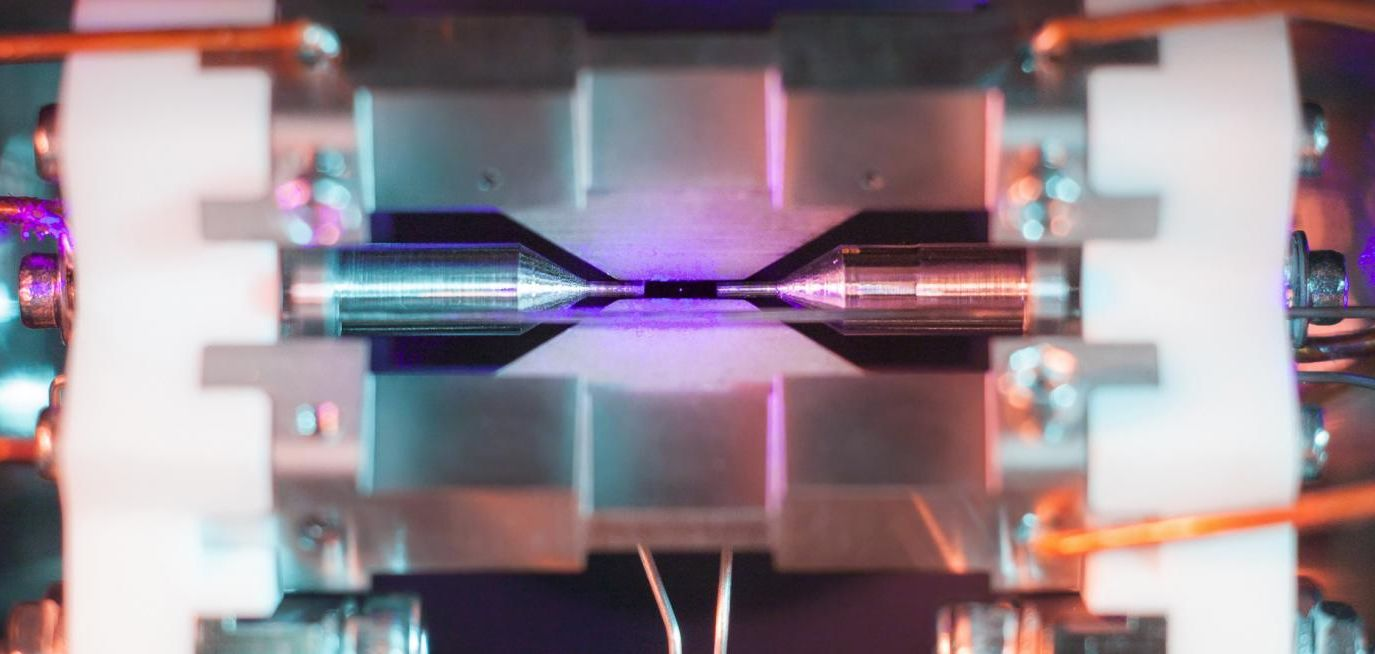
\includegraphics[width=0.95\linewidth]{TIQC.jpg}\\
			\vspace*{-.5em}\\
			\parbox{\linewidth}{\centering\footnotesize A trapped ion at the University of Oxford Ion trap quantum computing research group. Picture taken from their website\footnotemark.}
		\end{tabular}
	\vspace*{-0.75em}
\end{wrapfigure}

It is very important therefore to ensure that the qubits can be manipulated reliably. To achieve this one needs a relatively stable quantum state that can be used as the qubits and some stable way of sharing information between, manipulating and measuring these qubits to implement quantum algorithms reliably. A promising avenue toward implementation is by using trapped ions. These are charged atomic particles that are confined using magnetic and electric fields. Their internal electronic structure is ideal for use as qubits, while their back and forth motion in the trap is shared between all the ions present. As these ions are cooled to a few millionths of a Kelvin above absolute zero, this motion takes on a quantum nature, meaning that the ions' motion will only have discrete energies. This makes it a very convenient way of facilitating entanglement between them. Combination of Lasers addressing the ions can then be used to facilitate transfer between the various qubit states.

In our MSci project, we simulated how different combinations of lasers, called driving schemes, can improve the reliability of a quantum computer. We did this to set expectations and give guidance to an upcoming experiment, where these schemes will be tested on a physical system. Because of this our main focus was how we can mitigate against experimental errors that inevitably arise and reduce the reliability of the qubits' state. These come from a variety of sources like the temperature and degree to which the ions can be confined. To find the best setup for the experiment we evaluated different driving schemes aimed to address the specific problems a physical system might face and have given recommendation on which ones to use. We also shown that several of these schemes could be combined giving improved performance. We hope that the increased reliability of these schemes will be demonstrated in the following years.%While these issues can be mitigated by using specific driving schemes, those only usually address a single problem each. For this reason, we also developed a combination of two distinct driving schemes and demonstrated that this can reduce the noise to the qubits. We hope that in the following years this work may be continued by experimentally demonstrating the improvement our driving scheme can provide.
}
\vspace*{\fill}

\footnotetext[1]{\href{https://www.physics.ox.ac.uk/research/group/ion-trap-quantum-computing}{https://www.physics.ox.ac.uk/research/group/ion-trap-quantum-computing}}
\newpage

\fancyhead[RE,LO]{}
%%%%%%%%%%%%%%%%%%%%%%%%%%%%%%%%%%%schemes%
\newcounter{abstractpage}
\setcounter{abstractpage}{\value{page}}

\begin{abstract}
\thispagestyle{fancy}
\setcounter{page}{\value{abstractpage}}

	
\setcounter{abstractpage}{\value{page}}
\end{abstract}

\setcounter{page}{\value{abstractpage}}
\stepcounter{page}
\newpage
%%%%%%%%%%%%%%%%%%%%%%%%%%%%%%%%%%%%
%\section*{Acknowledgments}

\vspace*{\fill}
\begin{center}
	\textbf{Acknowledgements}\\

\end{center}
\vspace*{\fill}
%Comment this out if not needed.
\newpage
%\clearpage{\pagestyle{empty}}

%%%%%%%%%%%%%%%%%%%%%%%%%%%%%%%%%%%%
%--- table of contents
\fancyhead[RE,LO]{\sffamily {Table of Contents}}
\tableofcontents
\listoffigures
%\listoftables 

\clearpage{\pagestyle{empty}\cleardoublepage}
\pagenumbering{arabic}
\setcounter{page}{1}
\fancyhead[LE,RO]{\slshape \rightmark}
\fancyhead[LO,RE]{\slshape \leftmark}

%%%%%%%%%%%%%%%%%%%%%%%%%%%%%%%%%%%%
\chapter{Introduction}
\label{Intro}

%%%%%%%%%%%%%%%%%%%%%%%%%%%%%%%%%%%%
\chapter{Background}
\label{Background}

\section{Radio-frequency trap}
\label{Background:RF_Trap}

To understand the operation of trapped ion quantum computers, we have to examine how they are implemented and what properties do these systems have. The trap we are interested in is a so called radio-frequency (RF) or Paul trap \cite{RF_Traps, Charged_Particle_traps_Paul}. As pictured in \figref{fig:rftrap:schematic} this design uses several electrodes to create an oscillating potential, which induces a trapping force on charged particles. The stability, design and construction of these traps is extensively documented in literature \cite{Charged_Particle_traps_Paul,RF_Traps} and because these subtleties are not important to the respected gate designs these will not be further discussed here.

For our purposes we can treat the ions' electronic structure as a two level system with transition frequency $\omega_0$. This allows us to express the Hamiltonian of many ions in a trap as \cite{RF_Traps}:

\begin{align}
	\hat{H} &= \sum_{i} \frac{\hbar \omega_0}{2}\hat{\sigma}_z^{\left(i\right)} + \hbar\nu\left(\hat{a}^\dagger\hat{a} + \frac{1}{2}\right)
	\label{eq:RF_Trap_H}\\
	\hat{H} &= \frac{\hbar \omega_0}{2}\hat{S}_z + \hbar\nu\left(\hat{a}^\dagger\hat{a} + \frac{1}{2}\right)
	\label{eq:RF_Trap_H_S}
\end{align}

The first term of course corresponds to the ions simplified energy structure. We have used $\hat{\sigma}_j^{\left(i\right)}$ to signal the $j$th Pauli matrix acting on the $i$th ion. We have also introduced $\hat{S}_j \equiv \sum_{i} \hat{\sigma}_j^{\left(i\right)}$. The second term then is the shared vibrational motion of the ions. Adding an array of monochromatic laser driving terms, each with frequency $\omega_j$ and wavenumber $\mathbf{k}_j$, this becomes:

\begin{equation}
	\hat{H} = \frac{\hbar \omega_0}{2}\hat{S}_z + \hbar\nu\left(\hat{a}^\dagger\hat{a} + \frac{1}{2}\right) + \sum_{j}\frac{\hbar\Omega_j}{2}\hat{\sigma}^{\left(n_j\right)}_+\left(e^{-i\left(\mathbf{k}_j\mathbf{\hat{z}} - \omega_jt\right)} + h.c.\right) + h.c.
	\label{eq:RF_Trap_H_driven}
\end{equation}

Here $\Omega_j$ is the usual definition of the Rabi frequency \cite{Foot} and the $j$th laser addresses the $n_j$th ion. By using $\mathbf{\hat{z}} = \mathbf{z_0}\left(\hat{a} + \hat{a}^\dagger\right)$, where $\mathbf{z_0}$ is the ground state spread of the wavefunction $\mathbf{z_0} = \langle0|\mathbf{\hat{z}}|0\rangle$. This can then be used to define the Lamb-dicke parameter\cite{Sideband_cooling_penning_trap} as $\eta_j\equiv\mathbf{k}_j\mathbf{z_0}$. As we will see later this can be used to quantify the coupling of our laser to the trap's motional mode. Using this we can rewrite the previous Hamiltonian as:

\begin{equation}
	\hat{H} = \frac{\hbar \omega_0}{2}\hat{S}_z + \hbar\nu\left(\hat{a}^\dagger\hat{a} + \frac{1}{2}\right) + \sum_{j}\frac{\hbar\Omega_j}{2}\hat{\sigma}^{\left(n_j\right)}_+\left(e^{-i\left(\eta_j\left(\hat{a} + \hat{a}^\dagger\right) - \omega_jt\right)} + h.c.\right) + h.c.
	\label{eq:RF_Trap_H_driven_LD_param}
\end{equation}

We can then move into the interaction picture with respect to the first two terms. Defining $\hat{\tilde{a}}\equiv\hat{a}e^{i\nu t}$ and $\hat{\tilde{a}}^\dagger\equiv\hat{a}^\dagger e^{-i\nu t}$ and disregarding the fast oscillating terms we can write the new Hamiltonian as:

%\begin{wrapfigure}{r}{0.5\linewidth}
\begin{figure}[t!]
	\centering
	\begin{subfigure}[t]{0.4\textwidth}
		\centering
		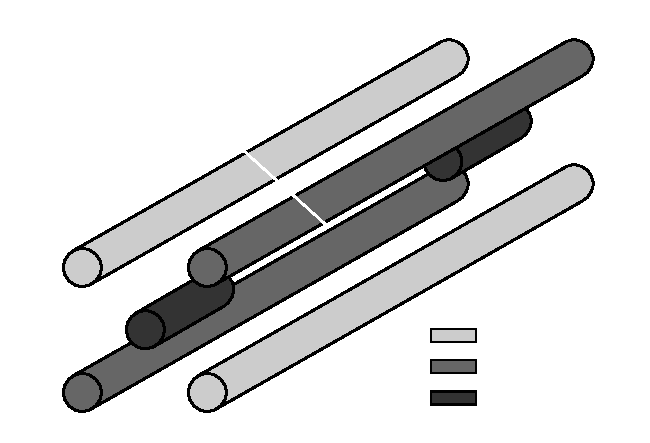
\includegraphics[width=\textwidth]{RF_Trap.pdf}
		\caption{A schematic representation of a simple RF trap. The four electrodes and two endcaps provide the trapping potential.}
		\label{fig:rftrap:schematic}
	\end{subfigure}
	\hfill
	\begin{subfigure}[t]{0.55\textwidth}
		\centering
		
\includegraphics[width=\textwidth]{1ion_Elevels.pdf}
		\caption{Simplified energy structure of an ion in the trap. The qubit states are separated by $\omega_0$ while the motional modes' spacing is dependent on the RF trap's frequency $\nu$.}
		\label{fig:rftrap:estructure}
	\end{subfigure}
	%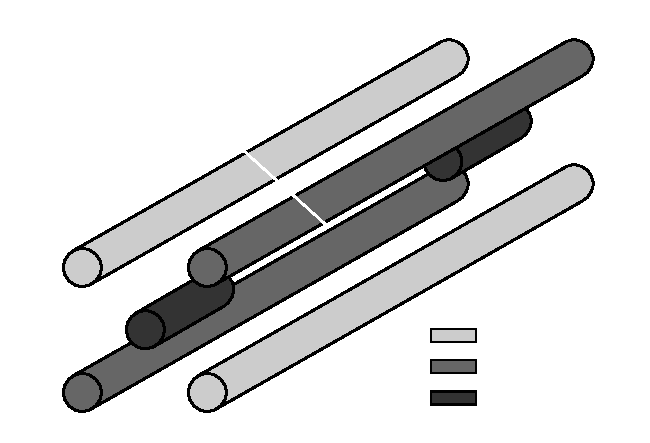
\includegraphics[width=0.7\linewidth]{RF_Trap.pdf}
	\caption[RF Trap schematic and energy]{The static field generated by the endcaps is combined with a fast oscillating field to provide confinement. This usually organises the ions on the trap's axis in a string like pattern \cite{RF_Traps,Charged_Particle_traps_Paul}. This creates an electronic structure pictured in \figref{fig:rftrap:estructure}.}
	\label{fig:rftrap}
\end{figure}
%\end{wrapfigure}

\begin{equation}
	\hat{H}_I = \sum_{j}\frac{\hbar\Omega_j}{2}\hat{\sigma}^{\left(n_j\right)}_+e^{i\eta_j\left(\hat{\tilde{a}} + \hat{\tilde{a}}^\dagger\right)} e^{-i\Delta_jt} + h.c.
	\label{eq:Interaction_H}
\end{equation}

Here we defined $\Delta_j\equiv\omega_j-\omega_0$. We can further examine this Hamiltonian by applying the Lamb-Dicke regime approximation, which is valid for $\langle\eta_j\hat{a}^\dagger\rangle \ll 1$ \cite{MS_gate}. In this limit, we can replace our exponential with the first order expansion, yielding the Hamiltonian:

\begin{equation}
	\hat{H}_I = \sum_{j}\frac{\hbar\Omega_j}{2}\hat{\sigma}^{\left(n_j\right)}_+\left(\mathds{1} + i\eta_j\left(\hat{\tilde{a}} + \hat{\tilde{a}}^\dagger\right)\right)e^{-i\Delta_jt} + h.c.
	\label{eq:Interaction_H_LD}
\end{equation}

This representation highlights two major issues about the system. The most obvious is that coupling to motional sidebands that used to share information between the ions \cite{QIP_Trapped_ions} heavily depends on the vibrational mode of the ions. This dependence will inevitably lead to decoherence of the qubit states, since the necessary timing will then differ for the various thermal occupations. This problem is further intensified by the RF trap's intrinsic property of heating \cite{QIP_Trapped_ions,RF_Traps}, which will lead to collapse of the motional mode if occurs so any entanglement of the qubits with the motional mode must be avoided.

The second issue is not as immediately obvious. This issue arises from the relative coupling strength of the carrier and the sideband transitions. While the central carrier transition will have coupling strength on the order of $\Omega_j$, an illuminating laser will only couple to the  $n$th sideband as an order of $\Omega_j\eta_j^n$. We will see later that this property leads to several unintended consequences.

\section{M\o lmer-S\o rensen gate}
\label{Background:MS_gate}

The M\o lmer-S\o rensen gate is a 

%%%%%%%%%%%%%%%%%%%%%%%%%%%%%%%%%%%%
\chapter{Explored driving schemes}
\label{Driving_schemes}

%%%%%%%%%%%%%%%%%%%%%%%%%%%%%%%%%%%%
\chapter{Dynamical decoupling}
\label{Dynamical_decoupling}

%%%%%%%%%%%%%%%%%%%%%%%%%%%%%%%%%%%%
\chapter{Conclusion}
\label{Conclusion}

%% bibliography
\bibliographystyle{ieeetran}
\bibliography{sources}

\end{document}